\documentclass{article}

\usepackage{filecontents}
\usepackage{tikz}
\usepackage{amsmath}
\usepackage{amsfonts}
\usepackage[bookmarks=true]{hyperref}
\input{util/util.tex}
\input{util/util-tikz.tex}
\input{util/theorem_proof_journal.tex}


\def\R{\ensuremath{\mathbb{R}}}
\begin{filecontents}{tmp.bib}
@book{boyd,
  title={\href{http://stanford.edu/~boyd/cvxbook/}{Convex Optimization}},
  author={Boyd, Stephen and Vandenberghe, Lieven},
  year={2004},
  publisher={Cambridge university press}
}

\end{filecontents}

\begin{document} 

\title{Geometry of quaders on top of surface elements of polytopes} 
\author{Andreas Orthey}
\date{}
\maketitle
\centering
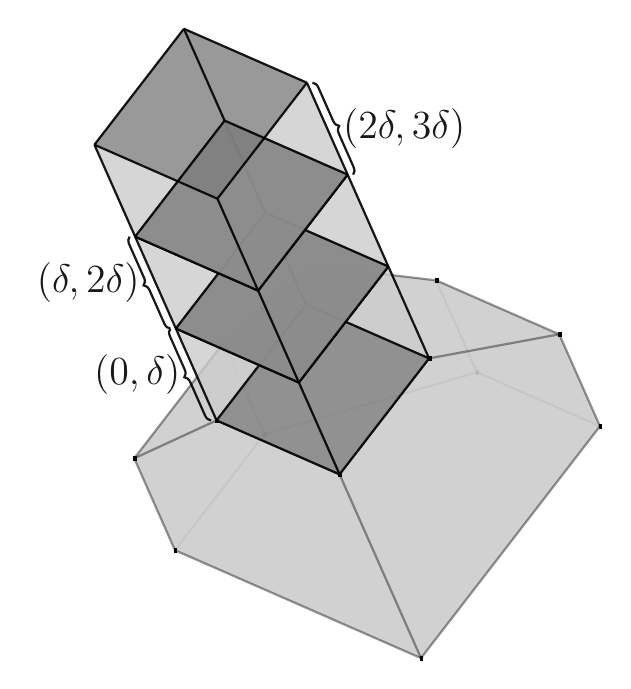
\begin{tikzpicture}%
        [x={(0.258520cm, -0.583496cm)},
        y={(0.781193cm, -0.342529cm)},
        z={(-0.568247cm, -0.736347cm)},
        scale=2.000000,
        back/.style={loosely dotted, thin},
        edge/.style={color=black, thick, opacity=0.4},
        circle/.style={color=white, thick, dashed},
        facet/.style={fill=black!20,color=black!20,fill opacity=0.9},
        specialFacet/.style={fill=black!20,color=black!80,fill opacity=0.9},
        boxfacet/.style={fill=black!30,color=black!50,fill opacity=0.8},
        boxside/.style={fill=black!30,color=black!20,fill opacity=0.8},
        boxedge/.style={color=black!100, thick, opacity=0.9},
        vertex/.style={inner sep=0.5pt,circle,draw=black!25!black,fill=black!75!black,thick,anchor=base},
        vertexC/.style={inner sep=5pt,circle,draw=black!100!black,fill=black!100!black,thick,anchor=base}]
%
%
%% Coordinate of the vertices:
%%

\coordinate (0.5, 0.5, -1.05) at (0.5, 0.5, 1.05);

\coordinate (-0.500, -0.500, -0.500) at (-0.500, -0.500, -0.500);
\coordinate (-1.00, 0.000, 0.000) at (-1.00, 0.000, 0.000);
\coordinate (-1.00, 0.000, 1.00) at (-1.00, 0.000, 1.00);
\coordinate (-1.00, 1.00, 0.000) at (-1.00, 1.00, 0.000);
\coordinate (-1.00, 1.00, 1.00) at (-1.00, 1.00, 1.00);
\coordinate (0.000, -1.00, 0.000) at (0.000, -1.00, 0.000);
\coordinate (0.000, -1.00, 1.00) at (0.000, -1.00, 1.00);
\coordinate (0.000, 0.000, -1.00) at (0.000, 0.000, -1.00);
\coordinate (0.000, 1.00, -1.00) at (0.000, 1.00, -1.00);
\coordinate (1.00, -1.00, 0.000) at (1.00, -1.00, 0.000);
\coordinate (1.00, -1.00, 1.00) at (1.00, -1.00, 1.00);
\coordinate (1.00, 0.000, -1.00) at (1.00, 0.000, -1.00);
\coordinate (1.00, 1.00, -1.00) at (1.00, 1.00, -1.00);
\coordinate (1.00, 1.00, 1.00) at (1.00, 1.00, 1.00);
%%
%%
%% Drawing edges in the back
%%
%%
%%
%% Drawing vertices in the back
%%
\node[vertex] at (1.00, -1.00, 0.000)     {};
\node[vertex] at (1.00, 0.000, -1.00)     {};
%%
%%
%% Drawing the facets
%%
\draw[edge] (0.000, -1.00, 0.000) -- (1.00, -1.00, 0.000);
\draw[edge] (0.000, 0.000, -1.00) -- (1.00, 0.000, -1.00);
\draw[edge] (1.00, 0.000, -1.00) -- (1.00, 1.00, -1.00);
\draw[edge] (1.00, -1.00, 0.000) -- (1.00, -1.00, 1.00);
\draw[edge] (1.00, -1.00, 0.000) -- (1.00, 0.000, -1.00);

\fill[facet] (1.00, 1.00, 1.00) -- (-1.00, 1.00, 1.00) -- (-1.00, 1.00, 0.000) -- (0.000, 1.00, -1.00) -- (1.00, 1.00, -1.00) -- cycle {};
\fill[facet] (1.00, 1.00, 1.00) -- (-1.00, 1.00, 1.00) -- (-1.00, 0.000, 1.00) -- (0.000, -1.00, 1.00) -- (1.00, -1.00, 1.00) -- cycle {};
\fill[facet] (0.000, -1.00, 1.00) -- (-1.00, 0.000, 1.00) -- (-1.00, 0.000, 0.000) -- (-0.500, -0.500, -0.500) -- (0.000, -1.00, 0.000) -- cycle {};
\fill[facet] (0.000, 1.00, -1.00) -- (-1.00, 1.00, 0.000) -- (-1.00, 0.000, 0.000) -- (-0.500, -0.500, -0.500) -- (0.000, 0.000, -1.00) -- cycle {};




\draw[edge] (1.00, -1.00, 1.00) -- (1.00, 1.00, 1.00);
\draw[edge] (1.00, 1.00, -1.00) -- (1.00, 1.00, 1.00);
\draw[edge] (0.000, -1.00, 1.00) -- (1.00, -1.00, 1.00);
\draw[edge] (0.000, 0.000, -1.00) -- (0.000, 1.00, -1.00);
\draw[edge] (0.000, 1.00, -1.00) -- (1.00, 1.00, -1.00);
%%
%%
%% Drawing edges in the front
%%
\draw[edge] (-0.500, -0.500, -0.500) -- (-1.00, 0.000, 0.000);
\draw[edge] (-0.500, -0.500, -0.500) -- (0.000, -1.00, 0.000);
\draw[edge] (-0.500, -0.500, -0.500) -- (0.000, 0.000, -1.00);
\draw[edge] (-1.00, 0.000, 0.000) -- (-1.00, 0.000, 1.00);
\draw[edge] (-1.00, 0.000, 0.000) -- (-1.00, 1.00, 0.000);
\draw[edge] (-1.00, 0.000, 1.00) -- (-1.00, 1.00, 1.00);
\draw[edge] (-1.00, 0.000, 1.00) -- (0.000, -1.00, 1.00);
\draw[edge] (-1.00, 1.00, 0.000) -- (-1.00, 1.00, 1.00);
\draw[edge] (-1.00, 1.00, 0.000) -- (0.000, 1.00, -1.00);
\draw[edge] (-1.00, 1.00, 1.00) -- (1.00, 1.00, 1.00);
\draw[edge] (0.000, -1.00, 0.000) -- (0.000, -1.00, 1.00);
%%
%%
%% Drawing the vertices in the front
%%
\node[vertex] at (-0.500, -0.500, -0.500)     {};
\node[vertex] at (-1.00, 0.000, 0.000)     {};
\node[vertex] at (-1.00, 0.000, 1.00)     {};
\node[vertex] at (-1.00, 1.00, 0.000)     {};
\node[vertex] at (-1.00, 1.00, 1.00)     {};
\node[vertex] at (0.000, -1.00, 0.000)     {};
\node[vertex] at (0.000, -1.00, 1.00)     {};
\node[vertex] at (0.000, 0.000, -1.00)     {};
\node[vertex] at (0.000, 1.00, -1.00)     {};
\node[vertex] at (1.00, -1.00, 1.00)     {};
\node[vertex] at (1.00, 1.00, -1.00)     {};
\node[vertex] at (1.00, 1.00, 1.00)     {};
%%
%\draw[circle] (-1.00, 0.50, 0.50) circle (11pt);
%\draw[thick,fill=white,color=white!80] (-1.00, 0.500, 0.500) circle (1pt) node[left] {$y$};
%\draw[fill=white,color=white] (-1.00, 0.500, 0.50) -- (-1.0,0.5,0.08) node[pos=0.3,right]{$R$};
\newcommand\drawBox[1]{
        \fill[boxside] (#1, 1.00, 1.00) -- (#1-1.0, 1.000, 1.00) -- (#1-1.0, 1.000, 0.000) -- (#1, 1.00, 0.000) -- cycle {};
        \fill[boxside] (#1-1.0, 1.00, 1.00) -- (#1-1.0, 0.000, 1.00) -- (#1, 0.000, 1.000) -- (#1, 1.00, 1.000) -- cycle {};
        \fill[boxfacet] (#1-1.0, 1.00, 1.00) -- (#1-1.0, 0.000, 1.00) -- (#1-1.0, 0.000, 0.000) -- (#1-1.0, 1.00, 0.000) -- cycle {};
        \fill[boxfacet] (#1, 1.00, 1.00) -- (#1, 0.000, 1.00) -- (#1, 0.000, 0.000) -- (#1, 1.00, 0.000) -- cycle {};

        \draw[boxedge] (#1-1.0, 1.00, 1.00) -- (#1, 1.00, 1.00);
        \draw[boxedge] (#1-1.0, 0.00, 1.00) -- (#1, 0.00, 1.00);
        \draw[boxedge] (#1-1.0, 0.00, 0.00) -- (#1, 0.00, 0.00);
        \draw[boxedge] (#1-1.0, 1.00, 0.00) -- (#1, 1.00, 0.00);
        \draw[boxedge] (#1, 1.00, 1.00) -- (#1, 0.00, 1.00);
        \draw[boxedge] (#1, 0.00, 1.00) -- (#1, 0.00, 0.00);
        \draw[boxedge] (#1, 0.00, 0.00) -- (#1, 1.00, 0.00);
        \draw[boxedge] (#1, 1.00, 0.00) -- (#1, 1.00, 1.00);
        \draw[boxedge] (#1-1.0, 1.00, 1.00) -- (#1-1.0, 0.00, 1.00);
        \draw[boxedge] (#1-1.0, 0.00, 1.00) -- (#1-1.0, 0.00, 0.00);
        \draw[boxedge] (#1-1.0, 0.00, 0.00) -- (#1-1.0, 1.00, 0.00);
        \draw[boxedge] (#1-1.0, 1.00, 0.00) -- (#1-1.0, 1.00, 1.00);
}
\def\hi{-1.00}
\drawBox{\hi}
\draw[boxedge,decoration={brace},decorate,xshift=-1pt] (\hi, 0.00, 1.00) --
(\hi-1.0, 0.00, 1.00) node[pos=0.5,left] {\Large $\bip(0,\delta)$}; 

\def \hi{-2.00}
\drawBox{\hi}
\draw[boxedge,decoration={brace},decorate,xshift=-1pt] (\hi, 0.00, 1.00) --
(\hi-1.0, 0.00, 1.00) node[pos=0.5,left] {\Large $\bip(\delta,2\delta)$}; 

\def\hi{-3.00}
\drawBox{\hi}
\draw[boxedge,decoration={brace},decorate,xshift=1pt] (\hi-1.0, 1.00, 0.00) --
(\hi, 1.00, 0.00) node[pos=0.5,right] {\Large $\bip(2\delta,3\delta)$};

\node at (-1.0, 0.6,0.3) {$\sip$};

\end{tikzpicture}



\begin{definition}
        Let an object $O_i$ be a convex bounded polytope 
        \begin{equation}
                \begin{aligned}
                        O_i=\{x\in \R^3| \ajit x\leq \bji, \|\aji\|_2=1,
                        j\in[1,M_i]\}
                \end{aligned}
        \end{equation}
        with $M_i$ the number of halfspaces.
\end{definition}

Let us take one surface element $\sip$ of $O_i$, given by
\begin{definition}[Surface Element]
        Given an object $O_i$, we call
        
        \begin{equation}
                \begin{aligned}
                        S_i^p = \{x \in \R^3|&\apit x = \bpi, \ajit x \leq \bji, \\
                                             &j=1,\cdots,p-1,p+1,\cdots,M_i\}
                \end{aligned}
        \end{equation}
        the $p$-th surface element of object $O_i$, and $\api$ is the
        surface normal with distance $\bpi$ to the origin.
\end{definition}

A quader on top of $\sip$ can now be defined as

\begin{definition}
        The quader $\bip(\Delta_L, \Delta_U)$ of height $\delta=\Delta_U-\Delta_L$ located
        with distance $\Delta_L$ above $\sip$ is defined as the set of points in

        \begin{equation}
                \begin{aligned}
                        \bip(\Delta_L, \Delta_U) = \{ x\in \R^3| -&\apit x \leq -\bpi-\Delta_L, \\
                                       &\apit x \leq \bpi + \Delta_U, \\
                                        &\ajipt x \leq \bjip,\\
                                        &{\scriptstyle j=1,\cdots,p-1,p+1,\cdots,M_i}\}
                \end{aligned}
        \end{equation}

        with $\ajip,\bjip$ belonging to the projected hyperplane $j$, with 
        
        \begin{equation}
                \begin{aligned}
                        \ajip &= \aji - (\ajit \api)\api\\
                        \bjip &= \ajipt \xji
                \end{aligned}
        \end{equation}
        whereby $\xji$ is one point on the intersection between hyperplane $H_j$
        and surface element $\sip$
        \begin{equation}
                \begin{aligned}
                        \xji \in \{x\in \R^3| &\ajit x = \bji, \\
                            &\akit y \leq \bki, \\
                            &{\scriptstyle k=1,\cdots,j-1,j+1,\cdots,p-1,p+1,\cdots,M_i}\}, \\
                            &\apit y = \bpi,\\
                            &\| x-y \|^2 = 0\}
                \end{aligned}
        \end{equation}
        Note that $x_0$ does not exist, if there is no common border between $\sip$ and
        $H_j$, in which case $\ajip,\bjip$ do not exist, i.e. they are not
        halfspace intersections of the box.
        %which corresponds to a rotation of the hyperplane, until $a_j' \perp
        %a_p$
\end{definition}


\bibliographystyle{plainnat}
\bibliography{tmp} 
\end{document}

